\documentclass[aspectratio=169]{beamer}
\mode<presentation>
%\usetheme{Warsaw}
%\usetheme{Goettingen}
\usetheme{Hannover}
%\useoutertheme{default}

%\useoutertheme{infolines}
\useoutertheme{sidebar}
\usecolortheme{dolphin}


\setbeamersize{sidebar width left=0pt} % to remove the sidebar
\beamertemplatenavigationsymbolsempty % To remove the navigation symbols on the bottom right.
\setbeamersize{text margin left=10mm,text margin right=10mm} % Specify margins

\usepackage{amsmath}
\usepackage{amssymb}
\usepackage{listings}
\usepackage{enumerate}
\usepackage{hyperref}
\hypersetup{
    colorlinks=true,
    linkcolor=blue,
    filecolor=magenta,      
    urlcolor=cyan,
}
 
\urlstyle{same}

%some bold math symbosl
\newcommand{\Cov}{\mathrm{Cov}}
\newcommand{\Var}{\mathrm{Var}}
\newcommand{\brho}{\boldsymbol{\rho}}
\newcommand{\bSigma}{\boldsymbol{\Sigma}}
\newcommand{\btheta}{\boldsymbol{\theta}}
\newcommand{\bbeta}{\boldsymbol{\beta}}
\newcommand{\bmu}{\boldsymbol{\mu}}
\newcommand{\bW}{\mathbf{W}}
\newcommand{\one}{\mathbf{1}}
\newcommand{\bH}{\mathbf{H}}
\newcommand{\by}{\mathbf{y}}
\newcommand{\bolde}{\mathbf{e}}
\newcommand{\bx}{\mathbf{x}}

\newcommand{\cpp}[1]{\texttt{#1}}

%--------------------------------------------------
\providecommand{\abs}[1]{\lvert#1\rvert}
\providecommand{\norm}[1]{\lVert#1\rVert}
\providecommand{\Blue}[1]{\textcolor{blue}{#1}}
\providecommand{\Red}[1]{\textcolor{red}{#1}}
\newcommand{\celsius}{\ensuremath{^\circ}C}
\newcommand\thfore{\mathord{\therefore}\,}
%--------------------------------------------


\title{Lecture 12. Propositional Logic}

%\author{
\includegraphics[width=.6\textwidth,height=.5\textheight]{lecture1-fig0.png} }
   
%\date{ {\tiny Figure Source: \url{http://web.csulb.edu/~cwallis/100/slides/toolkit/toolkit.html} } } 
\date{}


\begin{document}
\frame[plain]{\titlepage}


\begin{frame}[plain]{Terminology}
 
 {\bf Propositional logic - deals with statements}
 \medskip
 
 {\bf Propositional constants:}
 
   \begin{center}
    \begin{tabular}{ccc}
      T &-& True \\
      F &- & False
    \end{tabular}
   \end{center}

   {\bf Propositional variables} - can have T or F value.
  \medskip
  
  {\bf Simple statements:} They cannot be further subdivided.
 
    \begin{center} 
     ``The sun is shining."
    \end{center}
    
    \medskip
    
 {\bf Compound statements:} Not simple, contain at least one logical connective.
 \smallskip
 
 \begin{center}
   ``The sun is shining and the sky is blue."
 \end{center} 
  
 
\end{frame}


\begin{frame}[plain]{English to Logic}

\begin{itemize}
 \item  English  is often \Red{ambiguous}. 
   Translating sentences into \emph{symbols with logical connectives}~\footnote{Propositional logic}
   \Blue{removes the ambiguity}:
    \begin{enumerate}
       \item {\bf Identify} \emph{simple statements} and {\bf represent} using \emph{propositional  variables}  
       such  as  $p$, $q$, $r$....
       \item {\bf Determine} appropriate \emph{logical connectives}.
    \end{enumerate}\pause 
 \item {\bf Example 12.1.} Translate the following sentence into a \Blue{propositional form}:~\footnote{
   The propositional form is a compound statement with propositional variables (such as $p, q, r$) and
   logical connectives (such as $\wedge, \vee, \rightarrow$).}
   \smallskip
   
    \emph{
      ``\Blue{You can access the AI research lab \Red{if} you are a robotics specialist 
         or you are not a first-year student}."
         }\pause
         
%      ``\Blue{You can access the Internet from campus \Red{if} you are 
%      a computer science major \Red{or} you are \Red{not} a freshman}.''}\pause 
   \begin{itemize}
     \item {\bf a}: You can access the AI research lab. %
                    %You can access the Internet from campus.
     \item {\bf r}: You are a robotics specialist.
     %\item {\bf c}: You are a computer science major.
     \item {\bf f}: You are not a first-year student
                 %You are a freshman. \pause 
     \item Propositional logic: \Blue{$(r\vee \neg f)\rightarrow a$}
     \item Truth value of the propositional logic \\
         \begin{center}
         (Truth Table to the NEXT PAGE $\longrightarrow$ )
          \end{center}
   \end{itemize}
 \end{itemize}
\end{frame}

\begin{frame}[plain]{}

\begin{itemize}
     \item {\bf a}: You can access the AI research lab. %
                    %You can access the Internet from campus.
     \item {\bf r}: You are a robotics specialist.
     %\item {\bf c}: You are a computer science major.
     \item {\bf f}: You are not a first-year student
                 %You are a freshman. \pause 
     \item Propositional logic: \Blue{$(r\vee \neg f)\rightarrow a$}
\end{itemize}
  
         \begin{center}
        \begin{tabular}{|c|c|c|c|c|c|}\hline
          $r$ & $f$ & $a$ & $\neg f$ & $r\vee\neg f$ &  $(r\vee \neg f)\rightarrow a$ \\ \hline
            T  &  T  & T & F & T & \Blue{T}\\ \hline
            T  &  T  & F & F & T & \Blue{F}\\ \hline 
            T  &  F  & T & T & T & T\\ \hline
            T  &  F  & F & T & T & F\\ \hline
            F  &  T  & \Red{T} & F & \Red{F} & \Blue{T}\\ \hline
            F  &  T  & \Red{F} & F & \Red{F} & \Blue{T}\\ \hline
            F  &  F  & T & T & T & T\\ \hline
            F  &  F  & F & T & T & F\\ \hline
        \end{tabular}
	\end{center}\pause
	
{\bf Note}: This does not say anything about the fact \Red{when}
      $(r\vee \neg f)$ is \Red{false}, you \Red{might} or \Red{might not} have access.
      
\end{frame}

\begin{frame}[plain]{}

{\bf Practice 12.2.}
Translate the following statement into a propositional form and construct 
 its truth table:
   \smallskip
   
    \emph{
      ``You can't vote if you are under 18 years old or you are from Mars.''}
  
  \vspace{1.5in}
  
\end{frame}

\begin{frame}[plain]{Priority Order of Logic Operations}
 
 
 \begin{itemize}
   \item {\bf Parentheses}. Before operating on anything else, 
    you must evaluate all parentheticals starting at the innermost level.
     \begin{center}
       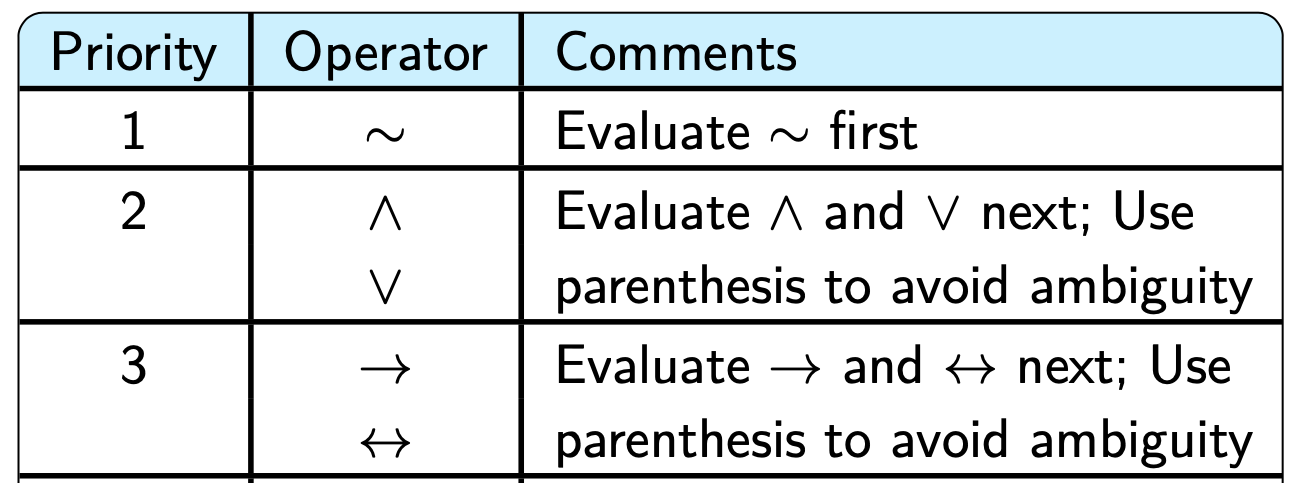
\includegraphics[height=3cm]{./img/lecture12-fig1.png}
    \end{center}
 \medskip
 
 
   \item {\bf Example 12.3}%~\footnote{Submit your answer at \textcolor{blue}{pollev.com/bongsikkim470}}   
  \  For each propositional logic in Python, indicate the value returned.
 \begin{itemize}
  \item $3 > 4 \ \Blue{\mathrm{or}}\ (2 < 3 \ \Blue{\mathrm{and}}\ 9 > 10)$ %False
  \item $4 > 5 \ \Blue{\mathrm{or}}\  3 < 4 \ \Blue{\mathrm{and}}\ 9 > 8$  % True
  \item $\neg ( 4 > 3 \ \Blue{\mathrm{and}}\ 100 > 6)$  % False
 \end{itemize}
 \end{itemize}
 
\end{frame}

\begin{frame}[plain]{}

 {\bf Practice 12.4} Consider the statement
   ``If Ahmed is late, then Mustafa is late, and, 
 if both Ahmed and Mustafa are late, then the class is boring."
 \smallskip
 
 Given the statement is True, if the class is not boring, 
 what can you conclude about Ahmed? 
    What about Mustafa?
%Essential, p26, sec 1.1, Example 1.3

\vspace{2in}

\end{frame}

\end{document}

%%%%%%%%%%%%%%%%%%%%%%%%%%%%%%%%%%%%%%


\begin{frame}[plain]{Exercises}

  \begin{enumerate}
 %   \item {\bf Knights and Knaves}\\
 %        \smallskip
          
% An island has two types of inhabitants: knights, who always tell
% the truth, and knaves, who always lie.  \\
% \smallskip

% You encounter two people, A and B.\\
% \smallskip

% Can you figure out what A and B are  
% if A says ``B is a knight'' and B says ``The two of us are opposite types?''

\item Build a digital circuit that produces the output $(p\vee\neg r)\wedge (\neg p\vee (q\vee \neg r))$
  when given input bits are $p, q,$ and $r$.
  
\item Determine the logical circuit for the given input-output table.
  \begin{center}
  \includegraphics[height=4.7cm]{lecture12-fig8.png}
 \end{center}
  

  \end{enumerate}
  
\end{frame}

\end{document}
    
